\chapter{Deployment Design}
\label{chap:deployment-design}

\section{Introduction}
The deployment architecture defines the physical hosting environment, network layout, continuous integration/continuous deployment (CI/CD) pipelines, and operational configurations for the Nexus PM platform. Designing a production environment requires balancing availability, data residency, latency, and resource constraints.

The deployment design for Nexus PM is built around containerized backend environments and edge-cached frontends, using managed cloud services to minimize operational maintenance. This chapter details the platform's multi-cloud infrastructure, deployment topologies, database connection rules, secure networks, environment variables, and deployment workflows.

\section{Cloud Infrastructure Overview}
Nexus PM uses a multi-cloud topology, deploying components to hosting providers based on their specific performance and billing characteristics. Table~\ref{tab:cloud_providers} summarizes the providers and their roles.

\begin{table}[h!]
\centering
\small
\renewcommand{\arraystretch}{1.4}
\begin{tabularx}{\textwidth}{l l X}
    \toprule[1.5pt]
    \rowcolor{primary!5}
    \textbf{\color{primary}Provider} & \textbf{\color{primary}Service Component} & \textbf{\color{primary}Operational Focus} \\
    \midrule
    \textbf{Vercel} & Frontend Web Client & Global CDN distribution, edge caching, and automated client builds. \\
    \textbf{Render} & Backend REST API Engine & Stateless Docker container hosting with health checks and logs. \\
    \textbf{Supabase} & Managed PostgreSQL Database & ACID storage, automated backups, and PgBouncer connection pooling. \\
    \textbf{Cloudflare} & R2 Object Storage & S3-compatible file storage with zero egress bandwidth charges. \\
    \textbf{Upstash} & Serverless Redis Cache & Serverless in-memory cache registry, session cache, and rate-limiting store. \\
    \textbf{Resend} & Email Gateway & API-driven transactional email dispatching. \\
    \bottomrule[1.5pt]
\end{tabularx}
\caption{Nexus PM Cloud Hosting Providers}
\label{tab:cloud_providers}
\end{table}

\section{Deployment Topology}
The runtime deployment topology is designed to secure communication and minimize latency between the client browser, API gateway, databases, and external cloud services, as shown in Figure~\ref{fig:deployment_topology}.

\begin{figure}[h!]
    \centering
    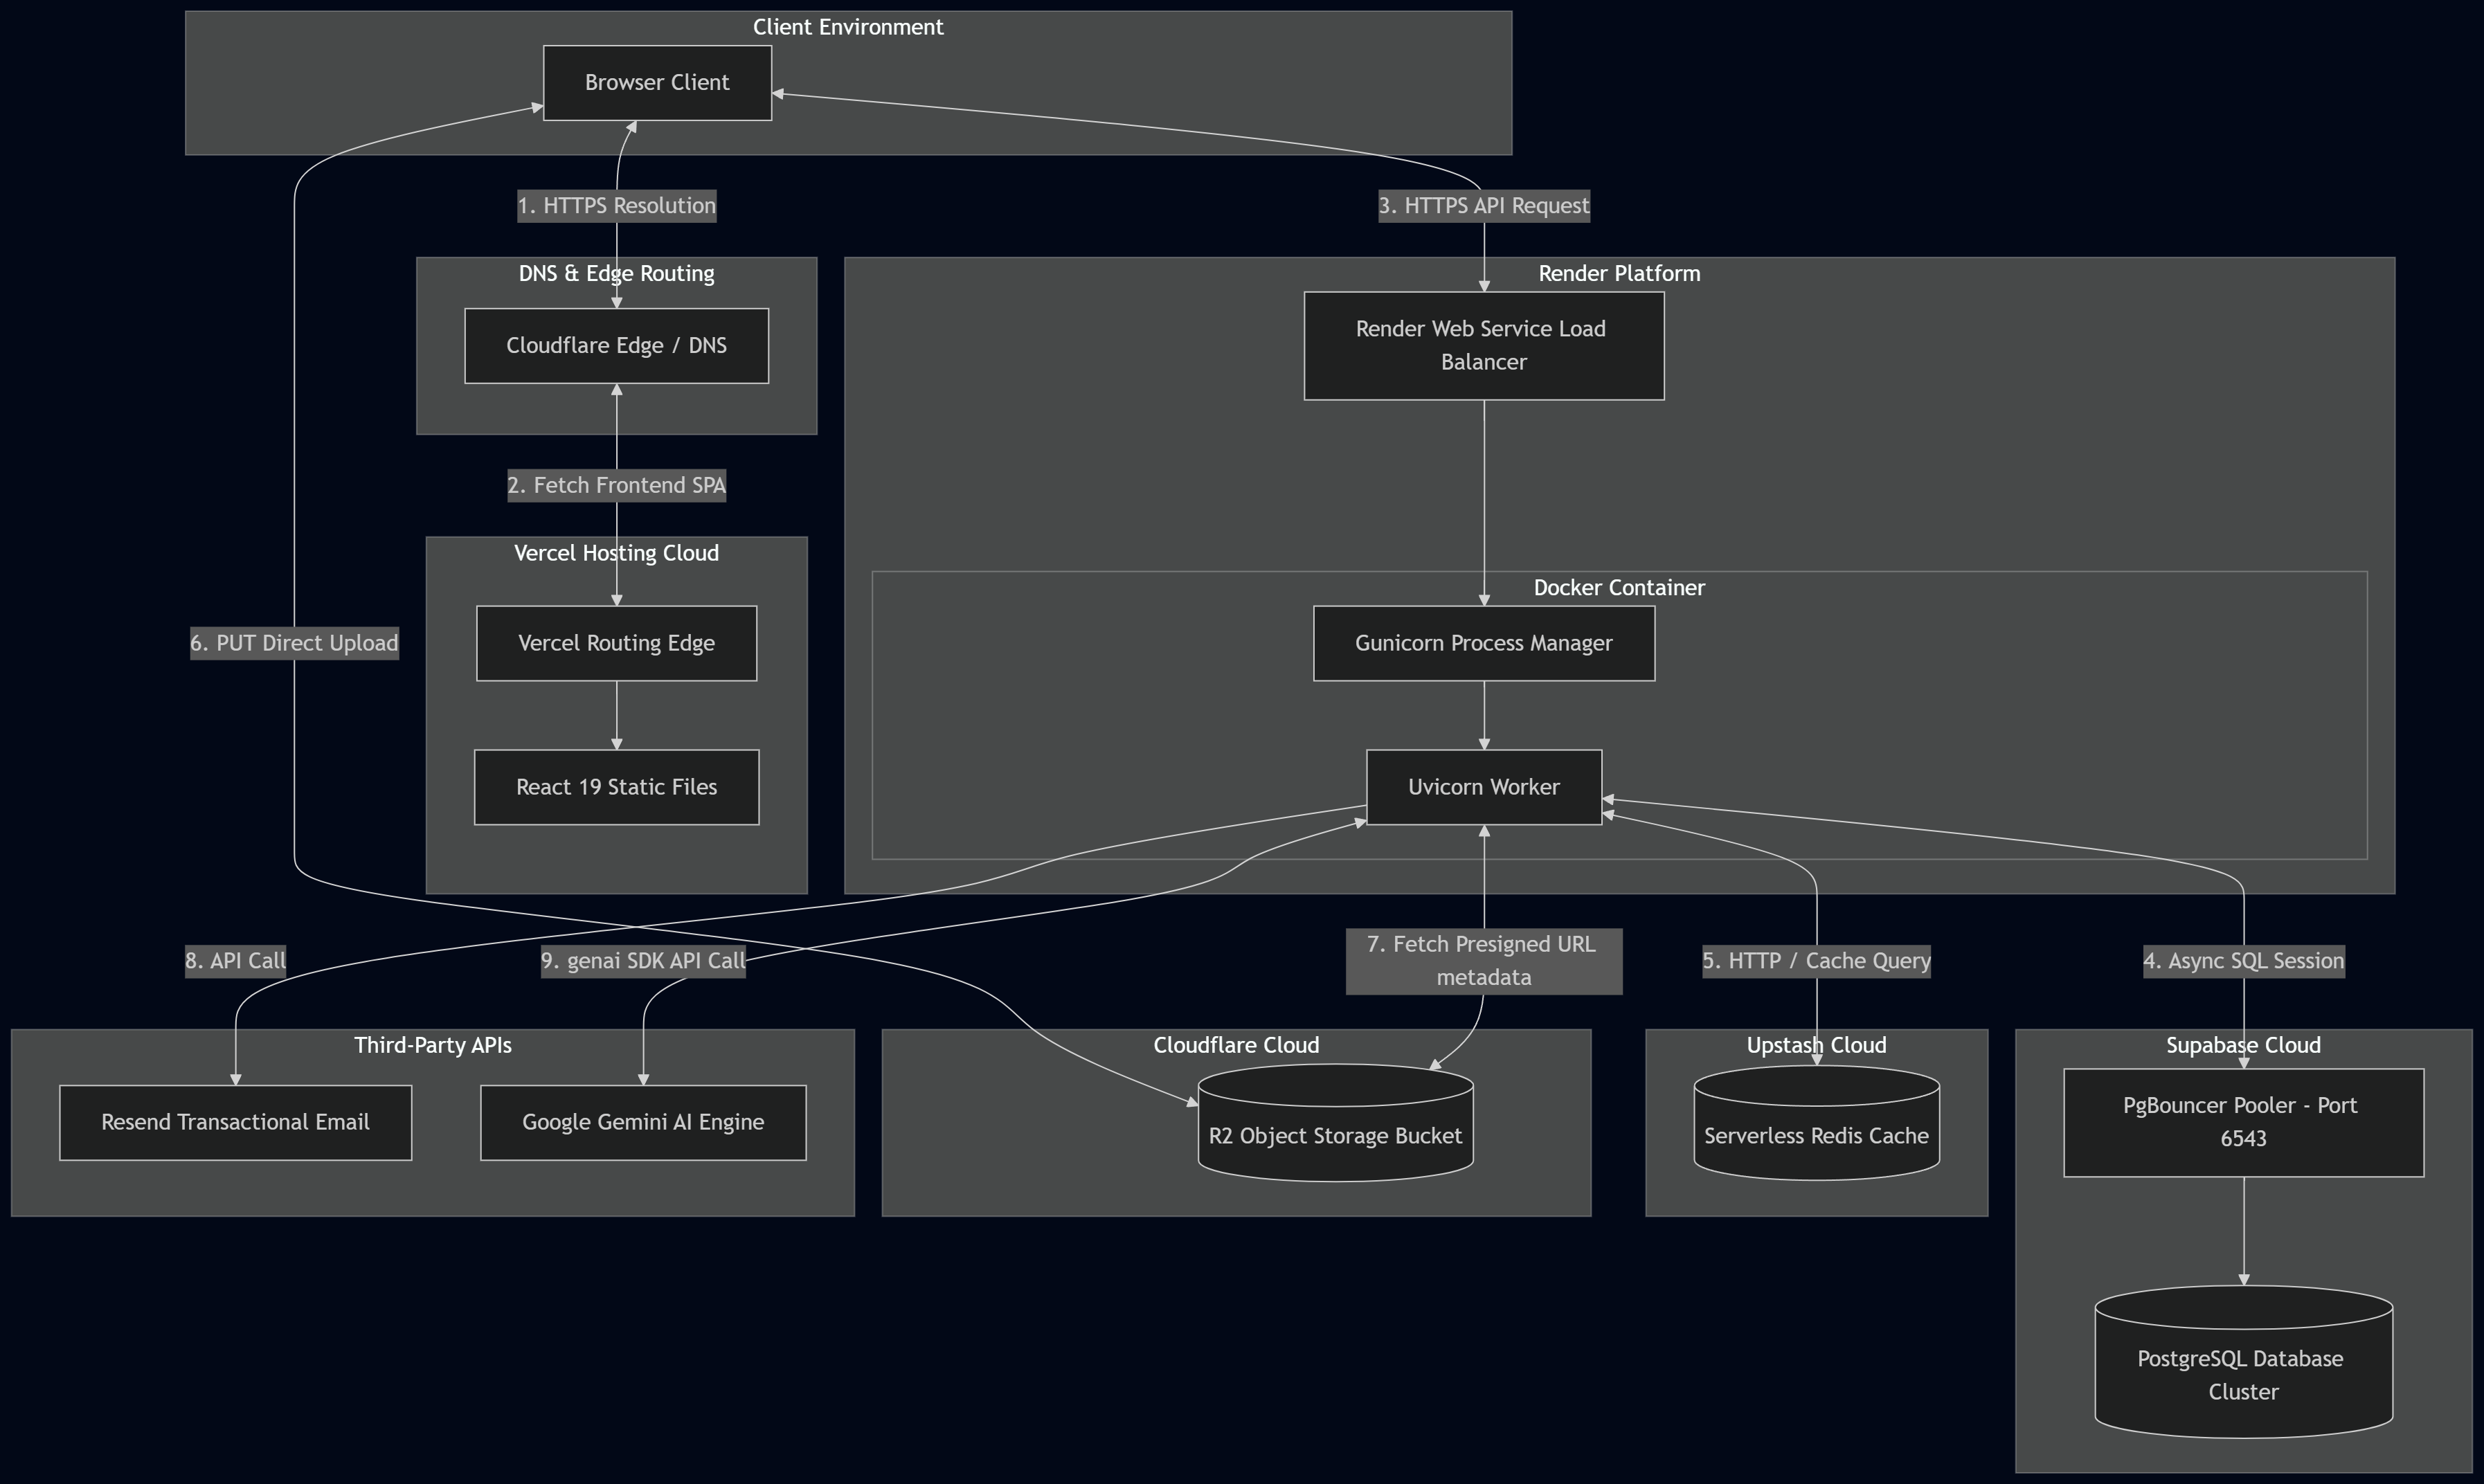
\includegraphics[width=\textwidth]{figures/deployment-architecture.png}
    \caption{Nexus PM Production Deployment Topology and Network Flow}
    \label{fig:deployment_topology}
\end{figure}

The division of hosting responsibilities between internal modules and external endpoints is outlined in Table~\ref{tab:deployment_responsibilities}.

\begin{table}[h!]
\centering
\small
\renewcommand{\arraystretch}{1.4}
\begin{tabularx}{\textwidth}{l l X}
    \toprule[1.5pt]
    \rowcolor{primary!5}
    \textbf{\color{primary}Service Layer} & \textbf{\color{primary}Deployment Node} & \textbf{\color{primary}Interface Responsibility} \\
    \midrule
    Presentation Client & Client Web Browser & Loads React static bundles from Vercel edge routers. \\
    API Controller & Render Docker Host & Decodes API requests, validates inputs, and coordinates services. \\
    Relational Storage & Supabase Database Node & Handles transactional SQL operations using PgBouncer. \\
    Cache Layer & Upstash Redis Node & Manages session states and rate limits. \\
    Asset Storage & Cloudflare R2 Bucket & Handles binary file transfers using pre-signed upload URLs. \\
    AI Reasoning & Google Gemini API Gateway & Processes prompt contexts asynchronously. \\
    Outbound SMTP & Resend Dispatch Node & Sends transaction alerts and workspace invitations. \\
    \bottomrule[1.5pt]
\end{tabularx}
\caption{Nexus PM Component Hosting Allocations}
\label{tab:deployment_responsibilities}
\end{table}

\section{Frontend Deployment}
The presentation layer is deployed to the \textbf{Vercel} platform as a compiled single-page application (SPA):
\begin{itemize}
    \item \textbf{Build Pipeline:} On code commits to the main repository, Vercel pulls the code, resolves dependencies, and compiles the React 19 codebase using Vite.
    \item \textbf{Edge Distribution:} The compiled HTML, CSS, and JS bundles are cached globally across Vercel's edge nodes. This routes initial client requests to the nearest edge location to minimize latency.
    \item \textbf{Routing and Caching:} Vercel handles client-side routing, falling back to \texttt{index.html} for unresolved paths to let the client routing framework handle transitions. Static resources are cached with long-lived HTTP headers to reduce traffic.
\end{itemize}

\section{Backend Deployment}
The API backend is hosted on \textbf{Render} as a containerized web service:
\begin{itemize}
    \item \textbf{Docker Runtime:} The FastAPI service runs inside a lightweight Docker image based on \texttt{python:3.12-slim}. System dependencies (e.g., \texttt{libpq-dev}) are installed during build time.
    \item \textbf{Startup Routine:} The container uses \path{entrypoint.sh} to run database migrations (\texttt{alembic upgrade head}) before starting the web server. If migrations fail, the startup crashes, preventing the container from serving traffic with outdated schemas.
    \item \texttt{Uvicorn} handles ASGI routing inside the container, managed by a Gunicorn master process configured with a single worker worker to operate within Render's free-tier memory limits.
    \item \textbf{Cold Start Behavior:} On Render's free tier, containers enter sleep mode after 15 minutes of inactivity. Subsequent requests trigger a container rebuild and startup routine, causing a 30-50 second delay for the initial request.
\end{itemize}

\section{Database Deployment}
The database layer uses PostgreSQL hosted on \textbf{Supabase}:
\begin{itemize}
    \item \textbf{Connection Optimization:} Relational queries run over secure TCP connections. To manage database connection limits on the free tier, the API routes queries through a PgBouncer instance running in transaction-pooling mode.
    \item \textbf{Connection Pool Settings:} Because PgBouncer in transaction mode is incompatible with prepared statement caches, the SQLAlchemy database engine is configured with \texttt{"statement\_cache\_size": 0} to prevent query compilation errors.
    \item \textbf{Migrations and Backups:} Alembic upgrades run on container startup to keep the schema in sync. The database service schedules daily snapshot backups to support disaster recovery.
\end{itemize}

\section{Object Storage}
File attachments are stored in an S3-compatible bucket hosted on \textbf{Cloudflare R2}:
\begin{itemize}
    \item \textbf{Zero Egress Fees:} R2 was chosen to eliminate egress bandwidth fees, ensuring predictable operational costs as file volume grows.
    \item \textbf{Direct Upload Workflow:} The API generates pre-signed upload URLs, letting clients upload files directly to R2. This bypasses the backend API containers, saving compute resources and reducing network bottleneck risks.
    \item \textbf{Access Authorization:} Attachments are secured using unique file keys, and the backend validates task membership permissions before generating download links.
\end{itemize}

\section{Redis Cache}
In-memory caching is hosted on \textbf{Upstash Redis}:
\begin{itemize}
    \item \textbf{Rate Limiting:} API endpoints enforce rate limiting by tracking request counts per IP and user ID in Redis.
    \item \textbf{Serverless Deployment:} The serverless Redis cluster scales compute resources automatically based on traffic volume, avoiding the need to provision dedicated Redis nodes.
    \item \textbf{Session State Caching:} Redis caches active session tokens, checking revocations before validating access tokens.
\end{itemize}

\section{External Services}
Integrating external managed APIs keeps the application footprint low:
\begin{itemize}
    \item \textbf{Google OAuth Gateway} delegates authentication security, eliminating local credential storage risks.
    \item \textbf{Resend API} handles transactional email dispatches, offloading SMTP server maintenance.
    \item \textbf{Google Gemini API} provides Large Language Model capabilities, processing task generation requests.
\end{itemize}

\section{Networking}
Network configuration focuses on securing data transit:
\begin{itemize}
    \item \textbf{Domain Management:} The platform uses a custom domain (\texttt{nexuspm.online}). Vercel routes traffic, and Render secures the API gateway domain (\texttt{api.nexuspm.online}).
    \item \textbf{Transport Security:} All ingress and egress traffic must use HTTPS (TLS 1.3), preventing packet sniffing on public networks.
    \item \textbf{CORS Configuration:} Cross-Origin Resource Sharing (CORS) rules restrict access to the production frontend domain, blocking unauthorized browser requests.
\end{itemize}

\section{Environment Configuration}
Configuration settings are loaded dynamically from environment variables using Pydantic Settings classes. Table~\ref{tab:env_config} outlines the key settings used to configure the platform.

\begin{table}[h!]
\centering
\small
\renewcommand{\arraystretch}{1.4}
\begin{tabularx}{\textwidth}{l l X}
    \toprule[1.5pt]
    \rowcolor{primary!5}
    \textbf{\color{primary}Config Variable} & \textbf{\color{primary}Source} & \textbf{\color{primary}System Impact} \\
    \midrule
    \texttt{DATABASE\_URL} & Supabase & Connection string for the PostgreSQL database, routed through PgBouncer. \\
    \texttt{REDIS\_URL} & Upstash & Connection URI for the Redis cache. \\
    \texttt{SECRET\_KEY} & Local Key & Cryptographic key for signing local access tokens. \\
    \texttt{REFRESH\_SECRET\_KEY} & Local Key & Cryptographic key for signing refresh tokens. \\
    \texttt{R2\_BUCKET\_NAME} & Cloudflare & Name of the Cloudflare R2 storage bucket. \\
    \texttt{GEMINI\_API\_KEY} & Google & API key for authenticating Gemini AI requests. \\
    \texttt{RESEND\_API\_KEY} & Resend & API key for authenticating transactional email requests. \\
    \bottomrule[1.5pt]
\end{tabularx}
\caption{Key System Configuration Variables}
\label{tab:env_config}
\end{table}

\section{Deployment Pipeline}
The deployment pipeline uses automated Git integration to coordinate deployments:
\begin{enumerate}
    \item \textbf{Git Commit:} Developers push code updates to the central GitHub repository.
    \item \textbf{Frontend Build:} Vercel detects updates in the client codebase, compiles the static assets, and deploys the new version.
    \item \textbf{Backend Build:} Render detects updates in the backend codebase, pulls the source code, builds the Docker image, and deploys the container.
    \item \textbf{Migration Run:} The backend container runs the database migration script (\texttt{alembic upgrade head}) on startup, keeping the schema in sync before starting the API server.
\end{enumerate}

\section{Operational Considerations}
Operating the platform requires managing the trade-offs of free-tier hosting limits:
\begin{itemize}
    \item \textbf{Render Cold Starts:} Free-tier containers enter sleep mode after 15 minutes of inactivity. When a request is received, the container rebuilds and starts up, causing a 30-50 second delay. To keep the container active, automated ping services (e.g., cron jobs) trigger health checks every 10 minutes.
    \item \textbf{Logging and Diagnostics:} Backend logs are routed to Render's logging interface. The \texttt{X-Request-ID} trace header is appended to logs to support request tracing.
    \item \textbf{Disaster Recovery:} The managed database service schedules daily snapshot backups to support disaster recovery, while Cloudflare R2 replicates files across edge storage nodes.
\end{itemize}

\section{Future Improvements}
Future updates to the deployment architecture plan to address several scaling improvements:
\begin{itemize}
    \item \textbf{Infrastructure as Code (IaC):} Define system resources using tools like Terraform to automate infrastructure setups.
    \item \textbf{Dedicated Compute Nodes:} Migrate from free-tier containers to dedicated instances (e.g., AWS ECS or Kubernetes) to eliminate cold start delays.
    \item \textbf{Automated Secrets Management:} Move environment secrets to a managed vault service (e.g., AWS Secrets Manager) to secure key configurations.
\end{itemize}

\section{Chapter Summary}
This chapter detailed the deployment design for the Nexus PM platform, specifying its multi-cloud hosting, container configurations, database connection rules, and deployment pipelines. By combining Vercel CDN static deliveries, containerized Render web services, and managed cloud resources, the architecture delivers a scalable, cost-efficient hosting environment. The next chapter will outline the testing protocols used to verify this configuration.
